\clearpage

\section{Detailed study of the effect of systematics on the best-fit oscillation parameters}
\label{appendix:systematics_bestfit_oscillations}


This section describes a study into the effect of systematics on the best-fit oscillation parameters.
It was used to determine which systematic parameters to include in the 2+8 fit. Before doing the study, it was decided to include a systematic 
if its effect on the best-fit oscillation parameters is greater than one-quarter the size of the statistical error at one or more oscillation 
parameter points. The statistical error was evaluated using 2+0 fits of 10000 toy experiments with no systematic fluctuations at each 
oscillation parameter point. The oscillation parameter points used in this study are shown in Fig.\ \ref{fig:apdx:starplot_points}.

In the study, a 2+0 fit was done on a toy MC experiment created without statistical fluctuations and with a single systematic parameter 
tweaked by $\pm$1$\sigma$.
For correlated systematic parameters, $\sigma$ was defined as the square root of the corresponding covariance matrix diagonal entry.
The best-fit values of the oscillation parameters from the 2+0 fit are plotted as an arrow whose origin is at the input point of the study.
For ease of reading, no more than 11 systematics are included on a single plot; for this reason, the plots are split into the following categories:
\begin{itemize}
\item parameters used in the 2+8 fit, Figs. \ref{fig:apdx_star_important_0.80_0.0020}-\ref{fig:apdx_star_important_1.00_0.0030};
\item SuperK detector parameters, Figs. \ref{fig:apdx_star_sk_0.80_0.0020}-\ref{fig:apdx_star_sk_1.00_0.0030};
\item BANFF $\nu_\mu$ flux parameters, Figs. \ref{fig:apdx_star_banffnumu_0.80_0.0020}-\ref{fig:apdx_star_banffnumu_1.00_0.0030};
\item BANFF $\bar{\nu_\mu}$ flux parameters, Figs. \ref{fig:apdx_star_banffnumubar_0.80_0.0020}-\ref{fig:apdx_star_banffnumubar_1.00_0.0030};
\item BANFF cross section parameters, Figs. \ref{fig:apdx_star_banffxsec_0.80_0.0020}-\ref{fig:apdx_star_banffxsec_1.00_0.0030};
\item uncorrelated cross section parameters, Figs. \ref{fig:apdx_star_xsec_0.80_0.0020}-\ref{fig:apdx_star_xsec_1.00_0.0030};
\item FSI+SI parameters, Figs. \ref{fig:apdx_star_fsi_0.80_0.0020}-\ref{fig:apdx_star_fsi_1.00_0.0030};
\item non-23 sector oscillation parameters, Figs. \ref{fig:apdx_star_osc_0.80_0.0020}-\ref{fig:apdx_star_osc_1.00_0.0030}.
\end{itemize}

\begin{figure*}[htb]
\center
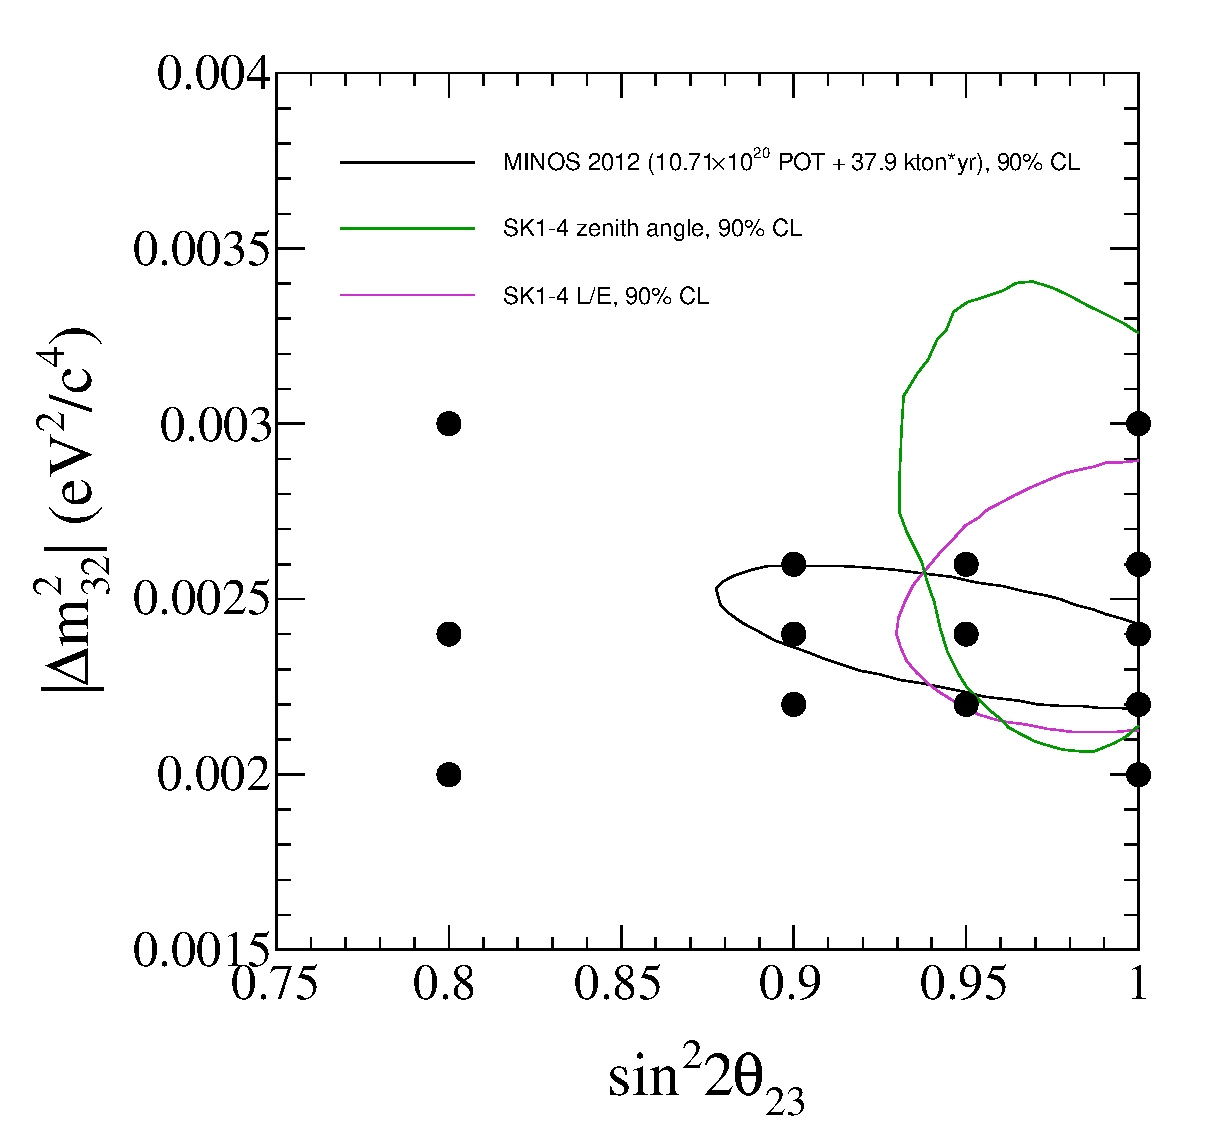
\includegraphics[width=25pc]{./images/star_plot/star_study_points}
\caption {
 True oscillation parameter points used in the study on the effect of systematics
 on the best-fit oscillation parameters.
}
\label{fig:apdx:starplot_points}
\end{figure*}


\clearpage


\subsection{Parameters used in the 2+8 fit}
\begin{figure*}[htb]
\begin{minipage}[t]{0.48\linewidth}
\center
\includegraphics[width=18pc]{{./images/star_plot/important-0.800000-0.002000_testbig}.eps}
\caption
{ Effect of parameters used in the 2+8 fit on the best fit point, using a 2+0 fit, with a single systematic changed by $\pm$1 sigma. The ellipse shown is one quarter the size of the statistical error. For 3 flavour oscillations, using oscillation parameters:  $\sin^22\theta_{12} = $0.857; $\sin^22\theta_{13} = $0.098; $\sin^22\theta_{23} = $0.8; $\delta_{CP} = $        0; $\Delta m^2_{12} = $    7.5e-05; $\Delta m^2_{32} = $    0.002. }
\label{fig:apdx_star_important_0.80_0.0020}
\end{minipage}
\hspace{0.06\linewidth}
\begin{minipage}[t]{0.48\linewidth}
\center
\includegraphics[width=18pc]{{./images/star_plot/important-0.800000-0.002400_testbig}.eps}
\caption
{ Effect of parameters used in the 2+8 fit on the best fit point, using a 2+0 fit, with a single systematic changed by $\pm$1 sigma. The ellipse shown is one quarter the size of the statistical error. For 3 flavour oscillations, using oscillation parameters:  $\sin^22\theta_{12} = $0.857; $\sin^22\theta_{13} = $0.098; $\sin^22\theta_{23} = $0.8; $\delta_{CP} = $        0; $\Delta m^2_{12} = $    7.5e-05; $\Delta m^2_{32} = $    0.0024. }
\label{fig:apdx_star_important_0.80_0.0024}
\end{minipage}
\vfill
\begin{minipage}[t]{0.48\linewidth}
\center
\includegraphics[width=18pc]{{./images/star_plot/important-0.800000-0.003000_testbig}.eps}
\caption
{ Effect of parameters used in the 2+8 fit on the best fit point, using a 2+0 fit, with a single systematic changed by $\pm$1 sigma. The ellipse shown is one quarter the size of the statistical error. For 3 flavour oscillations, using oscillation parameters:  $\sin^22\theta_{12} = $0.857; $\sin^22\theta_{13} = $0.098; $\sin^22\theta_{23} = $0.8; $\delta_{CP} = $        0; $\Delta m^2_{12} = $    7.5e-05; $\Delta m^2_{32} = $    0.003. }
\label{fig:apdx_star_important_0.80_0.0030}
\end{minipage}
\hspace{0.06\linewidth}
\begin{minipage}[t]{0.48\linewidth}
\center
\includegraphics[width=18pc]{{./images/star_plot/important-0.900000-0.002200_testbig}.eps}
\caption
{ Effect of parameters used in the 2+8 fit on the best fit point, using a 2+0 fit, with a single systematic changed by $\pm$1 sigma. The ellipse shown is one quarter the size of the statistical error. For 3 flavour oscillations, using oscillation parameters:  $\sin^22\theta_{12} = $0.857; $\sin^22\theta_{13} = $0.098; $\sin^22\theta_{23} = $0.9; $\delta_{CP} = $        0; $\Delta m^2_{12} = $    7.5e-05; $\Delta m^2_{32} = $    0.0022. }
\label{fig:apdx_star_important_0.90_0.0022}
\end{minipage}
\end{figure*}
\clearpage
\begin{figure*}[htb]
\begin{minipage}[t]{0.48\linewidth}
\center
\includegraphics[width=18pc]{{./images/star_plot/important-0.900000-0.002400_testbig}.eps}
\caption
{ Effect of parameters used in the 2+8 fit on the best fit point, using a 2+0 fit, with a single systematic changed by $\pm$1 sigma. The ellipse shown is one quarter the size of the statistical error. For 3 flavour oscillations, using oscillation parameters:  $\sin^22\theta_{12} = $0.857; $\sin^22\theta_{13} = $0.098; $\sin^22\theta_{23} = $0.9; $\delta_{CP} = $        0; $\Delta m^2_{12} = $    7.5e-05; $\Delta m^2_{32} = $    0.0024. }
\label{fig:apdx_star_important_0.90_0.0024}
\end{minipage}
\hspace{0.06\linewidth}
\begin{minipage}[t]{0.48\linewidth}
\center
\includegraphics[width=18pc]{{./images/star_plot/important-0.900000-0.002600_testbig}.eps}
\caption
{ Effect of parameters used in the 2+8 fit on the best fit point, using a 2+0 fit, with a single systematic changed by $\pm$1 sigma. The ellipse shown is one quarter the size of the statistical error. For 3 flavour oscillations, using oscillation parameters:  $\sin^22\theta_{12} = $0.857; $\sin^22\theta_{13} = $0.098; $\sin^22\theta_{23} = $0.9; $\delta_{CP} = $        0; $\Delta m^2_{12} = $    7.5e-05; $\Delta m^2_{32} = $    0.0026. }
\label{fig:apdx_star_important_0.90_0.0026}
\end{minipage}
\vfill
\begin{minipage}[t]{0.48\linewidth}
\center
\includegraphics[width=18pc]{{./images/star_plot/important-0.950000-0.002200_testbig}.eps}
\caption
{ Effect of parameters used in the 2+8 fit on the best fit point, using a 2+0 fit, with a single systematic changed by $\pm$1 sigma. The ellipse shown is one quarter the size of the statistical error. For 3 flavour oscillations, using oscillation parameters:  $\sin^22\theta_{12} = $0.857; $\sin^22\theta_{13} = $0.098; $\sin^22\theta_{23} = $0.95; $\delta_{CP} = $        0; $\Delta m^2_{12} = $    7.5e-05; $\Delta m^2_{32} = $    0.0022. }
\label{fig:apdx_star_important_0.95_0.0022}
\end{minipage}
\hspace{0.06\linewidth}
\begin{minipage}[t]{0.48\linewidth}
\center
\includegraphics[width=18pc]{{./images/star_plot/important-0.950000-0.002400_testbig}.eps}
\caption
{ Effect of parameters used in the 2+8 fit on the best fit point, using a 2+0 fit, with a single systematic changed by $\pm$1 sigma. The ellipse shown is one quarter the size of the statistical error. For 3 flavour oscillations, using oscillation parameters:  $\sin^22\theta_{12} = $0.857; $\sin^22\theta_{13} = $0.098; $\sin^22\theta_{23} = $0.95; $\delta_{CP} = $        0; $\Delta m^2_{12} = $    7.5e-05; $\Delta m^2_{32} = $    0.0024. }
\label{fig:apdx_star_important_0.95_0.0024}
\end{minipage}
\end{figure*}
\clearpage
\begin{figure*}[htb]
\begin{minipage}[t]{0.48\linewidth}
\center
\includegraphics[width=18pc]{{./images/star_plot/important-0.950000-0.002600_testbig}.eps}
\caption
{ Effect of parameters used in the 2+8 fit on the best fit point, using a 2+0 fit, with a single systematic changed by $\pm$1 sigma. The ellipse shown is one quarter the size of the statistical error. For 3 flavour oscillations, using oscillation parameters:  $\sin^22\theta_{12} = $0.857; $\sin^22\theta_{13} = $0.098; $\sin^22\theta_{23} = $0.95; $\delta_{CP} = $        0; $\Delta m^2_{12} = $    7.5e-05; $\Delta m^2_{32} = $    0.0026. }
\label{fig:apdx_star_important_0.95_0.0026}
\end{minipage}
\hspace{0.06\linewidth}
\begin{minipage}[t]{0.48\linewidth}
\center
\includegraphics[width=18pc]{{./images/star_plot/important-1.000000-0.002000_testbig}.eps}
\caption
{ Effect of parameters used in the 2+8 fit on the best fit point, using a 2+0 fit, with a single systematic changed by $\pm$1 sigma. The ellipse shown is one quarter the size of the statistical error. For 3 flavour oscillations, using oscillation parameters:  $\sin^22\theta_{12} = $0.857; $\sin^22\theta_{13} = $0.098; $\sin^22\theta_{23} = $1; $\delta_{CP} = $        0; $\Delta m^2_{12} = $    7.5e-05; $\Delta m^2_{32} = $    0.002. }
\label{fig:apdx_star_important_1.00_0.0020}
\end{minipage}
\vfill
\begin{minipage}[t]{0.48\linewidth}
\center
\includegraphics[width=18pc]{{./images/star_plot/important-1.000000-0.002200_testbig}.eps}
\caption
{ Effect of parameters used in the 2+8 fit on the best fit point, using a 2+0 fit, with a single systematic changed by $\pm$1 sigma. The ellipse shown is one quarter the size of the statistical error. For 3 flavour oscillations, using oscillation parameters:  $\sin^22\theta_{12} = $0.857; $\sin^22\theta_{13} = $0.098; $\sin^22\theta_{23} = $1; $\delta_{CP} = $        0; $\Delta m^2_{12} = $    7.5e-05; $\Delta m^2_{32} = $    0.0022. }
\label{fig:apdx_star_important_1.00_0.0022}
\end{minipage}
\hspace{0.06\linewidth}
\begin{minipage}[t]{0.48\linewidth}
\center
\includegraphics[width=18pc]{{./images/star_plot/important-1.000000-0.002400_testbig}.eps}
\caption
{ Effect of parameters used in the 2+8 fit on the best fit point, using a 2+0 fit, with a single systematic changed by $\pm$1 sigma. The ellipse shown is one quarter the size of the statistical error. For 3 flavour oscillations, using oscillation parameters:  $\sin^22\theta_{12} = $0.857; $\sin^22\theta_{13} = $0.098; $\sin^22\theta_{23} = $1; $\delta_{CP} = $        0; $\Delta m^2_{12} = $    7.5e-05; $\Delta m^2_{32} = $    0.0024. }
\label{fig:apdx_star_important_1.00_0.0024}
\end{minipage}
\end{figure*}
\clearpage
\begin{figure*}[htb]
\begin{minipage}[t]{0.48\linewidth}
\center
\includegraphics[width=18pc]{{./images/star_plot/important-1.000000-0.002600_testbig}.eps}
\caption
{ Effect of parameters used in the 2+8 fit on the best fit point, using a 2+0 fit, with a single systematic changed by $\pm$1 sigma. The ellipse shown is one quarter the size of the statistical error. For 3 flavour oscillations, using oscillation parameters:  $\sin^22\theta_{12} = $0.857; $\sin^22\theta_{13} = $0.098; $\sin^22\theta_{23} = $1; $\delta_{CP} = $        0; $\Delta m^2_{12} = $    7.5e-05; $\Delta m^2_{32} = $    0.0026. }
\label{fig:apdx_star_important_1.00_0.0026}
\end{minipage}
\hspace{0.06\linewidth}
\begin{minipage}[t]{0.48\linewidth}
\center
\includegraphics[width=18pc]{{./images/star_plot/important-1.000000-0.003000_testbig}.eps}
\caption
{ Effect of parameters used in the 2+8 fit on the best fit point, using a 2+0 fit, with a single systematic changed by $\pm$1 sigma. The ellipse shown is one quarter the size of the statistical error. For 3 flavour oscillations, using oscillation parameters:  $\sin^22\theta_{12} = $0.857; $\sin^22\theta_{13} = $0.098; $\sin^22\theta_{23} = $1; $\delta_{CP} = $        0; $\Delta m^2_{12} = $    7.5e-05; $\Delta m^2_{32} = $    0.003. }
\label{fig:apdx_star_important_1.00_0.0030}
\end{minipage}
\end{figure*}
\clearpage

\subsection{SuperK detector parameters}
\begin{figure*}[htb]
\begin{minipage}[t]{0.48\linewidth}
\center
\includegraphics[width=18pc]{{./images/star_plot/sk-0.800000-0.002000_testzoom}.eps}
\caption
{ Effect of SuperK detector parameters on the best fit point, using a 2+0 fit, with a single systematic changed by $\pm$1 sigma. The ellipse shown is one quarter the size of the statistical error. For 3 flavour oscillations, using oscillation parameters:  $\sin^22\theta_{12} = $0.857; $\sin^22\theta_{13} = $0.098; $\sin^22\theta_{23} = $0.8; $\delta_{CP} = $        0; $\Delta m^2_{12} = $    7.5e-05; $\Delta m^2_{32} = $    0.002. }
\label{fig:apdx_star_sk_0.80_0.0020}
\end{minipage}
\hspace{0.06\linewidth}
\begin{minipage}[t]{0.48\linewidth}
\center
\includegraphics[width=18pc]{{./images/star_plot/sk-0.800000-0.002400_testzoom}.eps}
\caption
{ Effect of SuperK detector parameters on the best fit point, using a 2+0 fit, with a single systematic changed by $\pm$1 sigma. The ellipse shown is one quarter the size of the statistical error. For 3 flavour oscillations, using oscillation parameters:  $\sin^22\theta_{12} = $0.857; $\sin^22\theta_{13} = $0.098; $\sin^22\theta_{23} = $0.8; $\delta_{CP} = $        0; $\Delta m^2_{12} = $    7.5e-05; $\Delta m^2_{32} = $    0.0024. }
\label{fig:apdx_star_sk_0.80_0.0024}
\end{minipage}
\vfill
\begin{minipage}[t]{0.48\linewidth}
\center
\includegraphics[width=18pc]{{./images/star_plot/sk-0.800000-0.003000_testzoom}.eps}
\caption
{ Effect of SuperK detector parameters on the best fit point, using a 2+0 fit, with a single systematic changed by $\pm$1 sigma. The ellipse shown is one quarter the size of the statistical error. For 3 flavour oscillations, using oscillation parameters:  $\sin^22\theta_{12} = $0.857; $\sin^22\theta_{13} = $0.098; $\sin^22\theta_{23} = $0.8; $\delta_{CP} = $        0; $\Delta m^2_{12} = $    7.5e-05; $\Delta m^2_{32} = $    0.003. }
\label{fig:apdx_star_sk_0.80_0.0030}
\end{minipage}
\hspace{0.06\linewidth}
\begin{minipage}[t]{0.48\linewidth}
\center
\includegraphics[width=18pc]{{./images/star_plot/sk-0.900000-0.002200_testzoom}.eps}
\caption
{ Effect of SuperK detector parameters on the best fit point, using a 2+0 fit, with a single systematic changed by $\pm$1 sigma. The ellipse shown is one quarter the size of the statistical error. For 3 flavour oscillations, using oscillation parameters:  $\sin^22\theta_{12} = $0.857; $\sin^22\theta_{13} = $0.098; $\sin^22\theta_{23} = $0.9; $\delta_{CP} = $        0; $\Delta m^2_{12} = $    7.5e-05; $\Delta m^2_{32} = $    0.0022. }
\label{fig:apdx_star_sk_0.90_0.0022}
\end{minipage}
\end{figure*}
\clearpage
\begin{figure*}[htb]
\begin{minipage}[t]{0.48\linewidth}
\center
\includegraphics[width=18pc]{{./images/star_plot/sk-0.900000-0.002400_testzoom}.eps}
\caption
{ Effect of SuperK detector parameters on the best fit point, using a 2+0 fit, with a single systematic changed by $\pm$1 sigma. The ellipse shown is one quarter the size of the statistical error. For 3 flavour oscillations, using oscillation parameters:  $\sin^22\theta_{12} = $0.857; $\sin^22\theta_{13} = $0.098; $\sin^22\theta_{23} = $0.9; $\delta_{CP} = $        0; $\Delta m^2_{12} = $    7.5e-05; $\Delta m^2_{32} = $    0.0024. }
\label{fig:apdx_star_sk_0.90_0.0024}
\end{minipage}
\hspace{0.06\linewidth}
\begin{minipage}[t]{0.48\linewidth}
\center
\includegraphics[width=18pc]{{./images/star_plot/sk-0.900000-0.002600_testzoom}.eps}
\caption
{ Effect of SuperK detector parameters on the best fit point, using a 2+0 fit, with a single systematic changed by $\pm$1 sigma. The ellipse shown is one quarter the size of the statistical error. For 3 flavour oscillations, using oscillation parameters:  $\sin^22\theta_{12} = $0.857; $\sin^22\theta_{13} = $0.098; $\sin^22\theta_{23} = $0.9; $\delta_{CP} = $        0; $\Delta m^2_{12} = $    7.5e-05; $\Delta m^2_{32} = $    0.0026. }
\label{fig:apdx_star_sk_0.90_0.0026}
\end{minipage}
\vfill
\begin{minipage}[t]{0.48\linewidth}
\center
\includegraphics[width=18pc]{{./images/star_plot/sk-0.950000-0.002200_testzoom}.eps}
\caption
{ Effect of SuperK detector parameters on the best fit point, using a 2+0 fit, with a single systematic changed by $\pm$1 sigma. The ellipse shown is one quarter the size of the statistical error. For 3 flavour oscillations, using oscillation parameters:  $\sin^22\theta_{12} = $0.857; $\sin^22\theta_{13} = $0.098; $\sin^22\theta_{23} = $0.95; $\delta_{CP} = $        0; $\Delta m^2_{12} = $    7.5e-05; $\Delta m^2_{32} = $    0.0022. }
\label{fig:apdx_star_sk_0.95_0.0022}
\end{minipage}
\hspace{0.06\linewidth}
\begin{minipage}[t]{0.48\linewidth}
\center
\includegraphics[width=18pc]{{./images/star_plot/sk-0.950000-0.002400_testzoom}.eps}
\caption
{ Effect of SuperK detector parameters on the best fit point, using a 2+0 fit, with a single systematic changed by $\pm$1 sigma. The ellipse shown is one quarter the size of the statistical error. For 3 flavour oscillations, using oscillation parameters:  $\sin^22\theta_{12} = $0.857; $\sin^22\theta_{13} = $0.098; $\sin^22\theta_{23} = $0.95; $\delta_{CP} = $        0; $\Delta m^2_{12} = $    7.5e-05; $\Delta m^2_{32} = $    0.0024. }
\label{fig:apdx_star_sk_0.95_0.0024}
\end{minipage}
\end{figure*}
\clearpage
\begin{figure*}[htb]
\begin{minipage}[t]{0.48\linewidth}
\center
\includegraphics[width=18pc]{{./images/star_plot/sk-0.950000-0.002600_testzoom}.eps}
\caption
{ Effect of SuperK detector parameters on the best fit point, using a 2+0 fit, with a single systematic changed by $\pm$1 sigma. The ellipse shown is one quarter the size of the statistical error. For 3 flavour oscillations, using oscillation parameters:  $\sin^22\theta_{12} = $0.857; $\sin^22\theta_{13} = $0.098; $\sin^22\theta_{23} = $0.95; $\delta_{CP} = $        0; $\Delta m^2_{12} = $    7.5e-05; $\Delta m^2_{32} = $    0.0026. }
\label{fig:apdx_star_sk_0.95_0.0026}
\end{minipage}
\hspace{0.06\linewidth}
\begin{minipage}[t]{0.48\linewidth}
\center
\includegraphics[width=18pc]{{./images/star_plot/sk-1.000000-0.002000_testzoom}.eps}
\caption
{ Effect of SuperK detector parameters on the best fit point, using a 2+0 fit, with a single systematic changed by $\pm$1 sigma. The ellipse shown is one quarter the size of the statistical error. For 3 flavour oscillations, using oscillation parameters:  $\sin^22\theta_{12} = $0.857; $\sin^22\theta_{13} = $0.098; $\sin^22\theta_{23} = $1; $\delta_{CP} = $        0; $\Delta m^2_{12} = $    7.5e-05; $\Delta m^2_{32} = $    0.002. }
\label{fig:apdx_star_sk_1.00_0.0020}
\end{minipage}
\vfill
\begin{minipage}[t]{0.48\linewidth}
\center
\includegraphics[width=18pc]{{./images/star_plot/sk-1.000000-0.002200_testzoom}.eps}
\caption
{ Effect of SuperK detector parameters on the best fit point, using a 2+0 fit, with a single systematic changed by $\pm$1 sigma. The ellipse shown is one quarter the size of the statistical error. For 3 flavour oscillations, using oscillation parameters:  $\sin^22\theta_{12} = $0.857; $\sin^22\theta_{13} = $0.098; $\sin^22\theta_{23} = $1; $\delta_{CP} = $        0; $\Delta m^2_{12} = $    7.5e-05; $\Delta m^2_{32} = $    0.0022. }
\label{fig:apdx_star_sk_1.00_0.0022}
\end{minipage}
\hspace{0.06\linewidth}
\begin{minipage}[t]{0.48\linewidth}
\center
\includegraphics[width=18pc]{{./images/star_plot/sk-1.000000-0.002400_testzoom}.eps}
\caption
{ Effect of SuperK detector parameters on the best fit point, using a 2+0 fit, with a single systematic changed by $\pm$1 sigma. The ellipse shown is one quarter the size of the statistical error. For 3 flavour oscillations, using oscillation parameters:  $\sin^22\theta_{12} = $0.857; $\sin^22\theta_{13} = $0.098; $\sin^22\theta_{23} = $1; $\delta_{CP} = $        0; $\Delta m^2_{12} = $    7.5e-05; $\Delta m^2_{32} = $    0.0024. }
\label{fig:apdx_star_sk_1.00_0.0024}
\end{minipage}
\end{figure*}
\clearpage
\begin{figure*}[htb]
\begin{minipage}[t]{0.48\linewidth}
\center
\includegraphics[width=18pc]{{./images/star_plot/sk-1.000000-0.002600_testzoom}.eps}
\caption
{ Effect of SuperK detector parameters on the best fit point, using a 2+0 fit, with a single systematic changed by $\pm$1 sigma. The ellipse shown is one quarter the size of the statistical error. For 3 flavour oscillations, using oscillation parameters:  $\sin^22\theta_{12} = $0.857; $\sin^22\theta_{13} = $0.098; $\sin^22\theta_{23} = $1; $\delta_{CP} = $        0; $\Delta m^2_{12} = $    7.5e-05; $\Delta m^2_{32} = $    0.0026. }
\label{fig:apdx_star_sk_1.00_0.0026}
\end{minipage}
\hspace{0.06\linewidth}
\begin{minipage}[t]{0.48\linewidth}
\center
\includegraphics[width=18pc]{{./images/star_plot/sk-1.000000-0.003000_testzoom}.eps}
\caption
{ Effect of SuperK detector parameters on the best fit point, using a 2+0 fit, with a single systematic changed by $\pm$1 sigma. The ellipse shown is one quarter the size of the statistical error. For 3 flavour oscillations, using oscillation parameters:  $\sin^22\theta_{12} = $0.857; $\sin^22\theta_{13} = $0.098; $\sin^22\theta_{23} = $1; $\delta_{CP} = $        0; $\Delta m^2_{12} = $    7.5e-05; $\Delta m^2_{32} = $    0.003. }
\label{fig:apdx_star_sk_1.00_0.0030}
\end{minipage}
\end{figure*}
\clearpage

\subsection{BANFF $\nu_\mu$ flux parameters}
\begin{figure*}[htb]
\begin{minipage}[t]{0.48\linewidth}
\center
\includegraphics[width=18pc]{{./images/star_plot/banffnumu-0.800000-0.002000_testzoom}.eps}
\caption
{ Effect of BANFF $\nu_\mu$ flux parameters on the best fit point, using a 2+0 fit, with a single systematic changed by $\pm$1 sigma. The ellipse shown is one quarter the size of the statistical error. For 3 flavour oscillations, using oscillation parameters:  $\sin^22\theta_{12} = $0.857; $\sin^22\theta_{13} = $0.098; $\sin^22\theta_{23} = $0.8; $\delta_{CP} = $        0; $\Delta m^2_{12} = $    7.5e-05; $\Delta m^2_{32} = $    0.002. }
\label{fig:apdx_star_banffnumu_0.80_0.0020}
\end{minipage}
\hspace{0.06\linewidth}
\begin{minipage}[t]{0.48\linewidth}
\center
\includegraphics[width=18pc]{{./images/star_plot/banffnumu-0.800000-0.002400_testzoom}.eps}
\caption
{ Effect of BANFF $\nu_\mu$ flux parameters on the best fit point, using a 2+0 fit, with a single systematic changed by $\pm$1 sigma. The ellipse shown is one quarter the size of the statistical error. For 3 flavour oscillations, using oscillation parameters:  $\sin^22\theta_{12} = $0.857; $\sin^22\theta_{13} = $0.098; $\sin^22\theta_{23} = $0.8; $\delta_{CP} = $        0; $\Delta m^2_{12} = $    7.5e-05; $\Delta m^2_{32} = $    0.0024. }
\label{fig:apdx_star_banffnumu_0.80_0.0024}
\end{minipage}
\vfill
\begin{minipage}[t]{0.48\linewidth}
\center
\includegraphics[width=18pc]{{./images/star_plot/banffnumu-0.800000-0.003000_testzoom}.eps}
\caption
{ Effect of BANFF $\nu_\mu$ flux parameters on the best fit point, using a 2+0 fit, with a single systematic changed by $\pm$1 sigma. The ellipse shown is one quarter the size of the statistical error. For 3 flavour oscillations, using oscillation parameters:  $\sin^22\theta_{12} = $0.857; $\sin^22\theta_{13} = $0.098; $\sin^22\theta_{23} = $0.8; $\delta_{CP} = $        0; $\Delta m^2_{12} = $    7.5e-05; $\Delta m^2_{32} = $    0.003. }
\label{fig:apdx_star_banffnumu_0.80_0.0030}
\end{minipage}
\hspace{0.06\linewidth}
\begin{minipage}[t]{0.48\linewidth}
\center
\includegraphics[width=18pc]{{./images/star_plot/banffnumu-0.900000-0.002200_testzoom}.eps}
\caption
{ Effect of BANFF $\nu_\mu$ flux parameters on the best fit point, using a 2+0 fit, with a single systematic changed by $\pm$1 sigma. The ellipse shown is one quarter the size of the statistical error. For 3 flavour oscillations, using oscillation parameters:  $\sin^22\theta_{12} = $0.857; $\sin^22\theta_{13} = $0.098; $\sin^22\theta_{23} = $0.9; $\delta_{CP} = $        0; $\Delta m^2_{12} = $    7.5e-05; $\Delta m^2_{32} = $    0.0022. }
\label{fig:apdx_star_banffnumu_0.90_0.0022}
\end{minipage}
\end{figure*}
\clearpage
\begin{figure*}[htb]
\begin{minipage}[t]{0.48\linewidth}
\center
\includegraphics[width=18pc]{{./images/star_plot/banffnumu-0.900000-0.002400_testzoom}.eps}
\caption
{ Effect of BANFF $\nu_\mu$ flux parameters on the best fit point, using a 2+0 fit, with a single systematic changed by $\pm$1 sigma. The ellipse shown is one quarter the size of the statistical error. For 3 flavour oscillations, using oscillation parameters:  $\sin^22\theta_{12} = $0.857; $\sin^22\theta_{13} = $0.098; $\sin^22\theta_{23} = $0.9; $\delta_{CP} = $        0; $\Delta m^2_{12} = $    7.5e-05; $\Delta m^2_{32} = $    0.0024. }
\label{fig:apdx_star_banffnumu_0.90_0.0024}
\end{minipage}
\hspace{0.06\linewidth}
\begin{minipage}[t]{0.48\linewidth}
\center
\includegraphics[width=18pc]{{./images/star_plot/banffnumu-0.900000-0.002600_testzoom}.eps}
\caption
{ Effect of BANFF $\nu_\mu$ flux parameters on the best fit point, using a 2+0 fit, with a single systematic changed by $\pm$1 sigma. The ellipse shown is one quarter the size of the statistical error. For 3 flavour oscillations, using oscillation parameters:  $\sin^22\theta_{12} = $0.857; $\sin^22\theta_{13} = $0.098; $\sin^22\theta_{23} = $0.9; $\delta_{CP} = $        0; $\Delta m^2_{12} = $    7.5e-05; $\Delta m^2_{32} = $    0.0026. }
\label{fig:apdx_star_banffnumu_0.90_0.0026}
\end{minipage}
\vfill
\begin{minipage}[t]{0.48\linewidth}
\center
\includegraphics[width=18pc]{{./images/star_plot/banffnumu-0.950000-0.002200_testzoom}.eps}
\caption
{ Effect of BANFF $\nu_\mu$ flux parameters on the best fit point, using a 2+0 fit, with a single systematic changed by $\pm$1 sigma. The ellipse shown is one quarter the size of the statistical error. For 3 flavour oscillations, using oscillation parameters:  $\sin^22\theta_{12} = $0.857; $\sin^22\theta_{13} = $0.098; $\sin^22\theta_{23} = $0.95; $\delta_{CP} = $        0; $\Delta m^2_{12} = $    7.5e-05; $\Delta m^2_{32} = $    0.0022. }
\label{fig:apdx_star_banffnumu_0.95_0.0022}
\end{minipage}
\hspace{0.06\linewidth}
\begin{minipage}[t]{0.48\linewidth}
\center
\includegraphics[width=18pc]{{./images/star_plot/banffnumu-0.950000-0.002400_testzoom}.eps}
\caption
{ Effect of BANFF $\nu_\mu$ flux parameters on the best fit point, using a 2+0 fit, with a single systematic changed by $\pm$1 sigma. The ellipse shown is one quarter the size of the statistical error. For 3 flavour oscillations, using oscillation parameters:  $\sin^22\theta_{12} = $0.857; $\sin^22\theta_{13} = $0.098; $\sin^22\theta_{23} = $0.95; $\delta_{CP} = $        0; $\Delta m^2_{12} = $    7.5e-05; $\Delta m^2_{32} = $    0.0024. }
\label{fig:apdx_star_banffnumu_0.95_0.0024}
\end{minipage}
\end{figure*}
\clearpage
\begin{figure*}[htb]
\begin{minipage}[t]{0.48\linewidth}
\center
\includegraphics[width=18pc]{{./images/star_plot/banffnumu-0.950000-0.002600_testzoom}.eps}
\caption
{ Effect of BANFF $\nu_\mu$ flux parameters on the best fit point, using a 2+0 fit, with a single systematic changed by $\pm$1 sigma. The ellipse shown is one quarter the size of the statistical error. For 3 flavour oscillations, using oscillation parameters:  $\sin^22\theta_{12} = $0.857; $\sin^22\theta_{13} = $0.098; $\sin^22\theta_{23} = $0.95; $\delta_{CP} = $        0; $\Delta m^2_{12} = $    7.5e-05; $\Delta m^2_{32} = $    0.0026. }
\label{fig:apdx_star_banffnumu_0.95_0.0026}
\end{minipage}
\hspace{0.06\linewidth}
\begin{minipage}[t]{0.48\linewidth}
\center
\includegraphics[width=18pc]{{./images/star_plot/banffnumu-1.000000-0.002000_testzoom}.eps}
\caption
{ Effect of BANFF $\nu_\mu$ flux parameters on the best fit point, using a 2+0 fit, with a single systematic changed by $\pm$1 sigma. The ellipse shown is one quarter the size of the statistical error. For 3 flavour oscillations, using oscillation parameters:  $\sin^22\theta_{12} = $0.857; $\sin^22\theta_{13} = $0.098; $\sin^22\theta_{23} = $1; $\delta_{CP} = $        0; $\Delta m^2_{12} = $    7.5e-05; $\Delta m^2_{32} = $    0.002. }
\label{fig:apdx_star_banffnumu_1.00_0.0020}
\end{minipage}
\vfill
\begin{minipage}[t]{0.48\linewidth}
\center
\includegraphics[width=18pc]{{./images/star_plot/banffnumu-1.000000-0.002200_testzoom}.eps}
\caption
{ Effect of BANFF $\nu_\mu$ flux parameters on the best fit point, using a 2+0 fit, with a single systematic changed by $\pm$1 sigma. The ellipse shown is one quarter the size of the statistical error. For 3 flavour oscillations, using oscillation parameters:  $\sin^22\theta_{12} = $0.857; $\sin^22\theta_{13} = $0.098; $\sin^22\theta_{23} = $1; $\delta_{CP} = $        0; $\Delta m^2_{12} = $    7.5e-05; $\Delta m^2_{32} = $    0.0022. }
\label{fig:apdx_star_banffnumu_1.00_0.0022}
\end{minipage}
\hspace{0.06\linewidth}
\begin{minipage}[t]{0.48\linewidth}
\center
\includegraphics[width=18pc]{{./images/star_plot/banffnumu-1.000000-0.002400_testzoom}.eps}
\caption
{ Effect of BANFF $\nu_\mu$ flux parameters on the best fit point, using a 2+0 fit, with a single systematic changed by $\pm$1 sigma. The ellipse shown is one quarter the size of the statistical error. For 3 flavour oscillations, using oscillation parameters:  $\sin^22\theta_{12} = $0.857; $\sin^22\theta_{13} = $0.098; $\sin^22\theta_{23} = $1; $\delta_{CP} = $        0; $\Delta m^2_{12} = $    7.5e-05; $\Delta m^2_{32} = $    0.0024. }
\label{fig:apdx_star_banffnumu_1.00_0.0024}
\end{minipage}
\end{figure*}
\clearpage
\begin{figure*}[htb]
\begin{minipage}[t]{0.48\linewidth}
\center
\includegraphics[width=18pc]{{./images/star_plot/banffnumu-1.000000-0.002600_testzoom}.eps}
\caption
{ Effect of BANFF $\nu_\mu$ flux parameters on the best fit point, using a 2+0 fit, with a single systematic changed by $\pm$1 sigma. The ellipse shown is one quarter the size of the statistical error. For 3 flavour oscillations, using oscillation parameters:  $\sin^22\theta_{12} = $0.857; $\sin^22\theta_{13} = $0.098; $\sin^22\theta_{23} = $1; $\delta_{CP} = $        0; $\Delta m^2_{12} = $    7.5e-05; $\Delta m^2_{32} = $    0.0026. }
\label{fig:apdx_star_banffnumu_1.00_0.0026}
\end{minipage}
\hspace{0.06\linewidth}
\begin{minipage}[t]{0.48\linewidth}
\center
\includegraphics[width=18pc]{{./images/star_plot/banffnumu-1.000000-0.003000_testzoom}.eps}
\caption
{ Effect of BANFF $\nu_\mu$ flux parameters on the best fit point, using a 2+0 fit, with a single systematic changed by $\pm$1 sigma. The ellipse shown is one quarter the size of the statistical error. For 3 flavour oscillations, using oscillation parameters:  $\sin^22\theta_{12} = $0.857; $\sin^22\theta_{13} = $0.098; $\sin^22\theta_{23} = $1; $\delta_{CP} = $        0; $\Delta m^2_{12} = $    7.5e-05; $\Delta m^2_{32} = $    0.003. }
\label{fig:apdx_star_banffnumu_1.00_0.0030}
\end{minipage}
\end{figure*}
\clearpage

\subsection{BANFF $\bar{\nu_\mu}$ flux parameters}
\begin{figure*}[htb]
\begin{minipage}[t]{0.48\linewidth}
\center
\includegraphics[width=18pc]{{./images/star_plot/banffnumubar-0.800000-0.002000_testzoom}.eps}
\caption
{ Effect of BANFF $\bar{\nu_\mu}$ flux parameters on the best fit point, using a 2+0 fit, with a single systematic changed by $\pm$1 sigma. The ellipse shown is one quarter the size of the statistical error. For 3 flavour oscillations, using oscillation parameters:  $\sin^22\theta_{12} = $0.857; $\sin^22\theta_{13} = $0.098; $\sin^22\theta_{23} = $0.8; $\delta_{CP} = $        0; $\Delta m^2_{12} = $    7.5e-05; $\Delta m^2_{32} = $    0.002. }
\label{fig:apdx_star_banffnumubar_0.80_0.0020}
\end{minipage}
\hspace{0.06\linewidth}
\begin{minipage}[t]{0.48\linewidth}
\center
\includegraphics[width=18pc]{{./images/star_plot/banffnumubar-0.800000-0.002400_testzoom}.eps}
\caption
{ Effect of BANFF $\bar{\nu_\mu}$ flux parameters on the best fit point, using a 2+0 fit, with a single systematic changed by $\pm$1 sigma. The ellipse shown is one quarter the size of the statistical error. For 3 flavour oscillations, using oscillation parameters:  $\sin^22\theta_{12} = $0.857; $\sin^22\theta_{13} = $0.098; $\sin^22\theta_{23} = $0.8; $\delta_{CP} = $        0; $\Delta m^2_{12} = $    7.5e-05; $\Delta m^2_{32} = $    0.0024. }
\label{fig:apdx_star_banffnumubar_0.80_0.0024}
\end{minipage}
\vfill
\begin{minipage}[t]{0.48\linewidth}
\center
\includegraphics[width=18pc]{{./images/star_plot/banffnumubar-0.800000-0.003000_testzoom}.eps}
\caption
{ Effect of BANFF $\bar{\nu_\mu}$ flux parameters on the best fit point, using a 2+0 fit, with a single systematic changed by $\pm$1 sigma. The ellipse shown is one quarter the size of the statistical error. For 3 flavour oscillations, using oscillation parameters:  $\sin^22\theta_{12} = $0.857; $\sin^22\theta_{13} = $0.098; $\sin^22\theta_{23} = $0.8; $\delta_{CP} = $        0; $\Delta m^2_{12} = $    7.5e-05; $\Delta m^2_{32} = $    0.003. }
\label{fig:apdx_star_banffnumubar_0.80_0.0030}
\end{minipage}
\hspace{0.06\linewidth}
\begin{minipage}[t]{0.48\linewidth}
\center
\includegraphics[width=18pc]{{./images/star_plot/banffnumubar-0.900000-0.002200_testzoom}.eps}
\caption
{ Effect of BANFF $\bar{\nu_\mu}$ flux parameters on the best fit point, using a 2+0 fit, with a single systematic changed by $\pm$1 sigma. The ellipse shown is one quarter the size of the statistical error. For 3 flavour oscillations, using oscillation parameters:  $\sin^22\theta_{12} = $0.857; $\sin^22\theta_{13} = $0.098; $\sin^22\theta_{23} = $0.9; $\delta_{CP} = $        0; $\Delta m^2_{12} = $    7.5e-05; $\Delta m^2_{32} = $    0.0022. }
\label{fig:apdx_star_banffnumubar_0.90_0.0022}
\end{minipage}
\end{figure*}
\clearpage
\begin{figure*}[htb]
\begin{minipage}[t]{0.48\linewidth}
\center
\includegraphics[width=18pc]{{./images/star_plot/banffnumubar-0.900000-0.002400_testzoom}.eps}
\caption
{ Effect of BANFF $\bar{\nu_\mu}$ flux parameters on the best fit point, using a 2+0 fit, with a single systematic changed by $\pm$1 sigma. The ellipse shown is one quarter the size of the statistical error. For 3 flavour oscillations, using oscillation parameters:  $\sin^22\theta_{12} = $0.857; $\sin^22\theta_{13} = $0.098; $\sin^22\theta_{23} = $0.9; $\delta_{CP} = $        0; $\Delta m^2_{12} = $    7.5e-05; $\Delta m^2_{32} = $    0.0024. }
\label{fig:apdx_star_banffnumubar_0.90_0.0024}
\end{minipage}
\hspace{0.06\linewidth}
\begin{minipage}[t]{0.48\linewidth}
\center
\includegraphics[width=18pc]{{./images/star_plot/banffnumubar-0.900000-0.002600_testzoom}.eps}
\caption
{ Effect of BANFF $\bar{\nu_\mu}$ flux parameters on the best fit point, using a 2+0 fit, with a single systematic changed by $\pm$1 sigma. The ellipse shown is one quarter the size of the statistical error. For 3 flavour oscillations, using oscillation parameters:  $\sin^22\theta_{12} = $0.857; $\sin^22\theta_{13} = $0.098; $\sin^22\theta_{23} = $0.9; $\delta_{CP} = $        0; $\Delta m^2_{12} = $    7.5e-05; $\Delta m^2_{32} = $    0.0026. }
\label{fig:apdx_star_banffnumubar_0.90_0.0026}
\end{minipage}
\vfill
\begin{minipage}[t]{0.48\linewidth}
\center
\includegraphics[width=18pc]{{./images/star_plot/banffnumubar-0.950000-0.002200_testzoom}.eps}
\caption
{ Effect of BANFF $\bar{\nu_\mu}$ flux parameters on the best fit point, using a 2+0 fit, with a single systematic changed by $\pm$1 sigma. The ellipse shown is one quarter the size of the statistical error. For 3 flavour oscillations, using oscillation parameters:  $\sin^22\theta_{12} = $0.857; $\sin^22\theta_{13} = $0.098; $\sin^22\theta_{23} = $0.95; $\delta_{CP} = $        0; $\Delta m^2_{12} = $    7.5e-05; $\Delta m^2_{32} = $    0.0022. }
\label{fig:apdx_star_banffnumubar_0.95_0.0022}
\end{minipage}
\hspace{0.06\linewidth}
\begin{minipage}[t]{0.48\linewidth}
\center
\includegraphics[width=18pc]{{./images/star_plot/banffnumubar-0.950000-0.002400_testzoom}.eps}
\caption
{ Effect of BANFF $\bar{\nu_\mu}$ flux parameters on the best fit point, using a 2+0 fit, with a single systematic changed by $\pm$1 sigma. The ellipse shown is one quarter the size of the statistical error. For 3 flavour oscillations, using oscillation parameters:  $\sin^22\theta_{12} = $0.857; $\sin^22\theta_{13} = $0.098; $\sin^22\theta_{23} = $0.95; $\delta_{CP} = $        0; $\Delta m^2_{12} = $    7.5e-05; $\Delta m^2_{32} = $    0.0024. }
\label{fig:apdx_star_banffnumubar_0.95_0.0024}
\end{minipage}
\end{figure*}
\clearpage
\begin{figure*}[htb]
\begin{minipage}[t]{0.48\linewidth}
\center
\includegraphics[width=18pc]{{./images/star_plot/banffnumubar-0.950000-0.002600_testzoom}.eps}
\caption
{ Effect of BANFF $\bar{\nu_\mu}$ flux parameters on the best fit point, using a 2+0 fit, with a single systematic changed by $\pm$1 sigma. The ellipse shown is one quarter the size of the statistical error. For 3 flavour oscillations, using oscillation parameters:  $\sin^22\theta_{12} = $0.857; $\sin^22\theta_{13} = $0.098; $\sin^22\theta_{23} = $0.95; $\delta_{CP} = $        0; $\Delta m^2_{12} = $    7.5e-05; $\Delta m^2_{32} = $    0.0026. }
\label{fig:apdx_star_banffnumubar_0.95_0.0026}
\end{minipage}
\hspace{0.06\linewidth}
\begin{minipage}[t]{0.48\linewidth}
\center
\includegraphics[width=18pc]{{./images/star_plot/banffnumubar-1.000000-0.002000_testzoom}.eps}
\caption
{ Effect of BANFF $\bar{\nu_\mu}$ flux parameters on the best fit point, using a 2+0 fit, with a single systematic changed by $\pm$1 sigma. The ellipse shown is one quarter the size of the statistical error. For 3 flavour oscillations, using oscillation parameters:  $\sin^22\theta_{12} = $0.857; $\sin^22\theta_{13} = $0.098; $\sin^22\theta_{23} = $1; $\delta_{CP} = $        0; $\Delta m^2_{12} = $    7.5e-05; $\Delta m^2_{32} = $    0.002. }
\label{fig:apdx_star_banffnumubar_1.00_0.0020}
\end{minipage}
\vfill
\begin{minipage}[t]{0.48\linewidth}
\center
\includegraphics[width=18pc]{{./images/star_plot/banffnumubar-1.000000-0.002200_testzoom}.eps}
\caption
{ Effect of BANFF $\bar{\nu_\mu}$ flux parameters on the best fit point, using a 2+0 fit, with a single systematic changed by $\pm$1 sigma. The ellipse shown is one quarter the size of the statistical error. For 3 flavour oscillations, using oscillation parameters:  $\sin^22\theta_{12} = $0.857; $\sin^22\theta_{13} = $0.098; $\sin^22\theta_{23} = $1; $\delta_{CP} = $        0; $\Delta m^2_{12} = $    7.5e-05; $\Delta m^2_{32} = $    0.0022. }
\label{fig:apdx_star_banffnumubar_1.00_0.0022}
\end{minipage}
\hspace{0.06\linewidth}
\begin{minipage}[t]{0.48\linewidth}
\center
\includegraphics[width=18pc]{{./images/star_plot/banffnumubar-1.000000-0.002400_testzoom}.eps}
\caption
{ Effect of BANFF $\bar{\nu_\mu}$ flux parameters on the best fit point, using a 2+0 fit, with a single systematic changed by $\pm$1 sigma. The ellipse shown is one quarter the size of the statistical error. For 3 flavour oscillations, using oscillation parameters:  $\sin^22\theta_{12} = $0.857; $\sin^22\theta_{13} = $0.098; $\sin^22\theta_{23} = $1; $\delta_{CP} = $        0; $\Delta m^2_{12} = $    7.5e-05; $\Delta m^2_{32} = $    0.0024. }
\label{fig:apdx_star_banffnumubar_1.00_0.0024}
\end{minipage}
\end{figure*}
\clearpage
\begin{figure*}[htb]
\begin{minipage}[t]{0.48\linewidth}
\center
\includegraphics[width=18pc]{{./images/star_plot/banffnumubar-1.000000-0.002600_testzoom}.eps}
\caption
{ Effect of BANFF $\bar{\nu_\mu}$ flux parameters on the best fit point, using a 2+0 fit, with a single systematic changed by $\pm$1 sigma. The ellipse shown is one quarter the size of the statistical error. For 3 flavour oscillations, using oscillation parameters:  $\sin^22\theta_{12} = $0.857; $\sin^22\theta_{13} = $0.098; $\sin^22\theta_{23} = $1; $\delta_{CP} = $        0; $\Delta m^2_{12} = $    7.5e-05; $\Delta m^2_{32} = $    0.0026. }
\label{fig:apdx_star_banffnumubar_1.00_0.0026}
\end{minipage}
\hspace{0.06\linewidth}
\begin{minipage}[t]{0.48\linewidth}
\center
\includegraphics[width=18pc]{{./images/star_plot/banffnumubar-1.000000-0.003000_testzoom}.eps}
\caption
{ Effect of BANFF $\bar{\nu_\mu}$ flux parameters on the best fit point, using a 2+0 fit, with a single systematic changed by $\pm$1 sigma. The ellipse shown is one quarter the size of the statistical error. For 3 flavour oscillations, using oscillation parameters:  $\sin^22\theta_{12} = $0.857; $\sin^22\theta_{13} = $0.098; $\sin^22\theta_{23} = $1; $\delta_{CP} = $        0; $\Delta m^2_{12} = $    7.5e-05; $\Delta m^2_{32} = $    0.003. }
\label{fig:apdx_star_banffnumubar_1.00_0.0030}
\end{minipage}
\end{figure*}
\clearpage

\subsection{BANFF cross section parameters}
\begin{figure*}[htb]
\begin{minipage}[t]{0.48\linewidth}
\center
\includegraphics[width=18pc]{{./images/star_plot/banffxsec-0.800000-0.002000_testzoom}.eps}
\caption
{ Effect of BANFF cross section parameters on the best fit point, using a 2+0 fit, with a single systematic changed by $\pm$1 sigma. The ellipse shown is one quarter the size of the statistical error. For 3 flavour oscillations, using oscillation parameters:  $\sin^22\theta_{12} = $0.857; $\sin^22\theta_{13} = $0.098; $\sin^22\theta_{23} = $0.8; $\delta_{CP} = $        0; $\Delta m^2_{12} = $    7.5e-05; $\Delta m^2_{32} = $    0.002. }
\label{fig:apdx_star_banffxsec_0.80_0.0020}
\end{minipage}
\hspace{0.06\linewidth}
\begin{minipage}[t]{0.48\linewidth}
\center
\includegraphics[width=18pc]{{./images/star_plot/banffxsec-0.800000-0.002400_testzoom}.eps}
\caption
{ Effect of BANFF cross section parameters on the best fit point, using a 2+0 fit, with a single systematic changed by $\pm$1 sigma. The ellipse shown is one quarter the size of the statistical error. For 3 flavour oscillations, using oscillation parameters:  $\sin^22\theta_{12} = $0.857; $\sin^22\theta_{13} = $0.098; $\sin^22\theta_{23} = $0.8; $\delta_{CP} = $        0; $\Delta m^2_{12} = $    7.5e-05; $\Delta m^2_{32} = $    0.0024. }
\label{fig:apdx_star_banffxsec_0.80_0.0024}
\end{minipage}
\vfill
\begin{minipage}[t]{0.48\linewidth}
\center
\includegraphics[width=18pc]{{./images/star_plot/banffxsec-0.800000-0.003000_testzoom}.eps}
\caption
{ Effect of BANFF cross section parameters on the best fit point, using a 2+0 fit, with a single systematic changed by $\pm$1 sigma. The ellipse shown is one quarter the size of the statistical error. For 3 flavour oscillations, using oscillation parameters:  $\sin^22\theta_{12} = $0.857; $\sin^22\theta_{13} = $0.098; $\sin^22\theta_{23} = $0.8; $\delta_{CP} = $        0; $\Delta m^2_{12} = $    7.5e-05; $\Delta m^2_{32} = $    0.003. }
\label{fig:apdx_star_banffxsec_0.80_0.0030}
\end{minipage}
\hspace{0.06\linewidth}
\begin{minipage}[t]{0.48\linewidth}
\center
\includegraphics[width=18pc]{{./images/star_plot/banffxsec-0.900000-0.002200_testzoom}.eps}
\caption
{ Effect of BANFF cross section parameters on the best fit point, using a 2+0 fit, with a single systematic changed by $\pm$1 sigma. The ellipse shown is one quarter the size of the statistical error. For 3 flavour oscillations, using oscillation parameters:  $\sin^22\theta_{12} = $0.857; $\sin^22\theta_{13} = $0.098; $\sin^22\theta_{23} = $0.9; $\delta_{CP} = $        0; $\Delta m^2_{12} = $    7.5e-05; $\Delta m^2_{32} = $    0.0022. }
\label{fig:apdx_star_banffxsec_0.90_0.0022}
\end{minipage}
\end{figure*}
\clearpage
\begin{figure*}[htb]
\begin{minipage}[t]{0.48\linewidth}
\center
\includegraphics[width=18pc]{{./images/star_plot/banffxsec-0.900000-0.002400_testzoom}.eps}
\caption
{ Effect of BANFF cross section parameters on the best fit point, using a 2+0 fit, with a single systematic changed by $\pm$1 sigma. The ellipse shown is one quarter the size of the statistical error. For 3 flavour oscillations, using oscillation parameters:  $\sin^22\theta_{12} = $0.857; $\sin^22\theta_{13} = $0.098; $\sin^22\theta_{23} = $0.9; $\delta_{CP} = $        0; $\Delta m^2_{12} = $    7.5e-05; $\Delta m^2_{32} = $    0.0024. }
\label{fig:apdx_star_banffxsec_0.90_0.0024}
\end{minipage}
\hspace{0.06\linewidth}
\begin{minipage}[t]{0.48\linewidth}
\center
\includegraphics[width=18pc]{{./images/star_plot/banffxsec-0.900000-0.002600_testzoom}.eps}
\caption
{ Effect of BANFF cross section parameters on the best fit point, using a 2+0 fit, with a single systematic changed by $\pm$1 sigma. The ellipse shown is one quarter the size of the statistical error. For 3 flavour oscillations, using oscillation parameters:  $\sin^22\theta_{12} = $0.857; $\sin^22\theta_{13} = $0.098; $\sin^22\theta_{23} = $0.9; $\delta_{CP} = $        0; $\Delta m^2_{12} = $    7.5e-05; $\Delta m^2_{32} = $    0.0026. }
\label{fig:apdx_star_banffxsec_0.90_0.0026}
\end{minipage}
\vfill
\begin{minipage}[t]{0.48\linewidth}
\center
\includegraphics[width=18pc]{{./images/star_plot/banffxsec-0.950000-0.002200_testzoom}.eps}
\caption
{ Effect of BANFF cross section parameters on the best fit point, using a 2+0 fit, with a single systematic changed by $\pm$1 sigma. The ellipse shown is one quarter the size of the statistical error. For 3 flavour oscillations, using oscillation parameters:  $\sin^22\theta_{12} = $0.857; $\sin^22\theta_{13} = $0.098; $\sin^22\theta_{23} = $0.95; $\delta_{CP} = $        0; $\Delta m^2_{12} = $    7.5e-05; $\Delta m^2_{32} = $    0.0022. }
\label{fig:apdx_star_banffxsec_0.95_0.0022}
\end{minipage}
\hspace{0.06\linewidth}
\begin{minipage}[t]{0.48\linewidth}
\center
\includegraphics[width=18pc]{{./images/star_plot/banffxsec-0.950000-0.002400_testzoom}.eps}
\caption
{ Effect of BANFF cross section parameters on the best fit point, using a 2+0 fit, with a single systematic changed by $\pm$1 sigma. The ellipse shown is one quarter the size of the statistical error. For 3 flavour oscillations, using oscillation parameters:  $\sin^22\theta_{12} = $0.857; $\sin^22\theta_{13} = $0.098; $\sin^22\theta_{23} = $0.95; $\delta_{CP} = $        0; $\Delta m^2_{12} = $    7.5e-05; $\Delta m^2_{32} = $    0.0024. }
\label{fig:apdx_star_banffxsec_0.95_0.0024}
\end{minipage}
\end{figure*}
\clearpage
\begin{figure*}[htb]
\begin{minipage}[t]{0.48\linewidth}
\center
\includegraphics[width=18pc]{{./images/star_plot/banffxsec-0.950000-0.002600_testzoom}.eps}
\caption
{ Effect of BANFF cross section parameters on the best fit point, using a 2+0 fit, with a single systematic changed by $\pm$1 sigma. The ellipse shown is one quarter the size of the statistical error. For 3 flavour oscillations, using oscillation parameters:  $\sin^22\theta_{12} = $0.857; $\sin^22\theta_{13} = $0.098; $\sin^22\theta_{23} = $0.95; $\delta_{CP} = $        0; $\Delta m^2_{12} = $    7.5e-05; $\Delta m^2_{32} = $    0.0026. }
\label{fig:apdx_star_banffxsec_0.95_0.0026}
\end{minipage}
\hspace{0.06\linewidth}
\begin{minipage}[t]{0.48\linewidth}
\center
\includegraphics[width=18pc]{{./images/star_plot/banffxsec-1.000000-0.002000_testzoom}.eps}
\caption
{ Effect of BANFF cross section parameters on the best fit point, using a 2+0 fit, with a single systematic changed by $\pm$1 sigma. The ellipse shown is one quarter the size of the statistical error. For 3 flavour oscillations, using oscillation parameters:  $\sin^22\theta_{12} = $0.857; $\sin^22\theta_{13} = $0.098; $\sin^22\theta_{23} = $1; $\delta_{CP} = $        0; $\Delta m^2_{12} = $    7.5e-05; $\Delta m^2_{32} = $    0.002. }
\label{fig:apdx_star_banffxsec_1.00_0.0020}
\end{minipage}
\vfill
\begin{minipage}[t]{0.48\linewidth}
\center
\includegraphics[width=18pc]{{./images/star_plot/banffxsec-1.000000-0.002200_testzoom}.eps}
\caption
{ Effect of BANFF cross section parameters on the best fit point, using a 2+0 fit, with a single systematic changed by $\pm$1 sigma. The ellipse shown is one quarter the size of the statistical error. For 3 flavour oscillations, using oscillation parameters:  $\sin^22\theta_{12} = $0.857; $\sin^22\theta_{13} = $0.098; $\sin^22\theta_{23} = $1; $\delta_{CP} = $        0; $\Delta m^2_{12} = $    7.5e-05; $\Delta m^2_{32} = $    0.0022. }
\label{fig:apdx_star_banffxsec_1.00_0.0022}
\end{minipage}
\hspace{0.06\linewidth}
\begin{minipage}[t]{0.48\linewidth}
\center
\includegraphics[width=18pc]{{./images/star_plot/banffxsec-1.000000-0.002400_testzoom}.eps}
\caption
{ Effect of BANFF cross section parameters on the best fit point, using a 2+0 fit, with a single systematic changed by $\pm$1 sigma. The ellipse shown is one quarter the size of the statistical error. For 3 flavour oscillations, using oscillation parameters:  $\sin^22\theta_{12} = $0.857; $\sin^22\theta_{13} = $0.098; $\sin^22\theta_{23} = $1; $\delta_{CP} = $        0; $\Delta m^2_{12} = $    7.5e-05; $\Delta m^2_{32} = $    0.0024. }
\label{fig:apdx_star_banffxsec_1.00_0.0024}
\end{minipage}
\end{figure*}
\clearpage
\begin{figure*}[htb]
\begin{minipage}[t]{0.48\linewidth}
\center
\includegraphics[width=18pc]{{./images/star_plot/banffxsec-1.000000-0.002600_testzoom}.eps}
\caption
{ Effect of BANFF cross section parameters on the best fit point, using a 2+0 fit, with a single systematic changed by $\pm$1 sigma. The ellipse shown is one quarter the size of the statistical error. For 3 flavour oscillations, using oscillation parameters:  $\sin^22\theta_{12} = $0.857; $\sin^22\theta_{13} = $0.098; $\sin^22\theta_{23} = $1; $\delta_{CP} = $        0; $\Delta m^2_{12} = $    7.5e-05; $\Delta m^2_{32} = $    0.0026. }
\label{fig:apdx_star_banffxsec_1.00_0.0026}
\end{minipage}
\hspace{0.06\linewidth}
\begin{minipage}[t]{0.48\linewidth}
\center
\includegraphics[width=18pc]{{./images/star_plot/banffxsec-1.000000-0.003000_testzoom}.eps}
\caption
{ Effect of BANFF cross section parameters on the best fit point, using a 2+0 fit, with a single systematic changed by $\pm$1 sigma. The ellipse shown is one quarter the size of the statistical error. For 3 flavour oscillations, using oscillation parameters:  $\sin^22\theta_{12} = $0.857; $\sin^22\theta_{13} = $0.098; $\sin^22\theta_{23} = $1; $\delta_{CP} = $        0; $\Delta m^2_{12} = $    7.5e-05; $\Delta m^2_{32} = $    0.003. }
\label{fig:apdx_star_banffxsec_1.00_0.0030}
\end{minipage}
\end{figure*}
\clearpage

\subsection{Uncorrelated cross section parameters}
\begin{figure*}[htb]
\begin{minipage}[t]{0.48\linewidth}
\center
\includegraphics[width=18pc]{{./images/star_plot/xsec-0.800000-0.002000_testzoom}.eps}
\caption
{ Effect of uncorrelated cross section parameters on the best fit point, using a 2+0 fit, with a single systematic changed by $\pm$1 sigma. The ellipse shown is one quarter the size of the statistical error. For 3 flavour oscillations, using oscillation parameters:  $\sin^22\theta_{12} = $0.857; $\sin^22\theta_{13} = $0.098; $\sin^22\theta_{23} = $0.8; $\delta_{CP} = $        0; $\Delta m^2_{12} = $    7.5e-05; $\Delta m^2_{32} = $    0.002. }
\label{fig:apdx_star_xsec_0.80_0.0020}
\end{minipage}
\hspace{0.06\linewidth}
\begin{minipage}[t]{0.48\linewidth}
\center
\includegraphics[width=18pc]{{./images/star_plot/xsec-0.800000-0.002400_testzoom}.eps}
\caption
{ Effect of uncorrelated cross section parameters on the best fit point, using a 2+0 fit, with a single systematic changed by $\pm$1 sigma. The ellipse shown is one quarter the size of the statistical error. For 3 flavour oscillations, using oscillation parameters:  $\sin^22\theta_{12} = $0.857; $\sin^22\theta_{13} = $0.098; $\sin^22\theta_{23} = $0.8; $\delta_{CP} = $        0; $\Delta m^2_{12} = $    7.5e-05; $\Delta m^2_{32} = $    0.0024. }
\label{fig:apdx_star_xsec_0.80_0.0024}
\end{minipage}
\vfill
\begin{minipage}[t]{0.48\linewidth}
\center
\includegraphics[width=18pc]{{./images/star_plot/xsec-0.800000-0.003000_testzoom}.eps}
\caption
{ Effect of uncorrelated cross section parameters on the best fit point, using a 2+0 fit, with a single systematic changed by $\pm$1 sigma. The ellipse shown is one quarter the size of the statistical error. For 3 flavour oscillations, using oscillation parameters:  $\sin^22\theta_{12} = $0.857; $\sin^22\theta_{13} = $0.098; $\sin^22\theta_{23} = $0.8; $\delta_{CP} = $        0; $\Delta m^2_{12} = $    7.5e-05; $\Delta m^2_{32} = $    0.003. }
\label{fig:apdx_star_xsec_0.80_0.0030}
\end{minipage}
\hspace{0.06\linewidth}
\begin{minipage}[t]{0.48\linewidth}
\center
\includegraphics[width=18pc]{{./images/star_plot/xsec-0.900000-0.002200_testzoom}.eps}
\caption
{ Effect of uncorrelated cross section parameters on the best fit point, using a 2+0 fit, with a single systematic changed by $\pm$1 sigma. The ellipse shown is one quarter the size of the statistical error. For 3 flavour oscillations, using oscillation parameters:  $\sin^22\theta_{12} = $0.857; $\sin^22\theta_{13} = $0.098; $\sin^22\theta_{23} = $0.9; $\delta_{CP} = $        0; $\Delta m^2_{12} = $    7.5e-05; $\Delta m^2_{32} = $    0.0022. }
\label{fig:apdx_star_xsec_0.90_0.0022}
\end{minipage}
\end{figure*}
\clearpage
\begin{figure*}[htb]
\begin{minipage}[t]{0.48\linewidth}
\center
\includegraphics[width=18pc]{{./images/star_plot/xsec-0.900000-0.002400_testzoom}.eps}
\caption
{ Effect of uncorrelated cross section parameters on the best fit point, using a 2+0 fit, with a single systematic changed by $\pm$1 sigma. The ellipse shown is one quarter the size of the statistical error. For 3 flavour oscillations, using oscillation parameters:  $\sin^22\theta_{12} = $0.857; $\sin^22\theta_{13} = $0.098; $\sin^22\theta_{23} = $0.9; $\delta_{CP} = $        0; $\Delta m^2_{12} = $    7.5e-05; $\Delta m^2_{32} = $    0.0024. }
\label{fig:apdx_star_xsec_0.90_0.0024}
\end{minipage}
\hspace{0.06\linewidth}
\begin{minipage}[t]{0.48\linewidth}
\center
\includegraphics[width=18pc]{{./images/star_plot/xsec-0.900000-0.002600_testzoom}.eps}
\caption
{ Effect of uncorrelated cross section parameters on the best fit point, using a 2+0 fit, with a single systematic changed by $\pm$1 sigma. The ellipse shown is one quarter the size of the statistical error. For 3 flavour oscillations, using oscillation parameters:  $\sin^22\theta_{12} = $0.857; $\sin^22\theta_{13} = $0.098; $\sin^22\theta_{23} = $0.9; $\delta_{CP} = $        0; $\Delta m^2_{12} = $    7.5e-05; $\Delta m^2_{32} = $    0.0026. }
\label{fig:apdx_star_xsec_0.90_0.0026}
\end{minipage}
\vfill
\begin{minipage}[t]{0.48\linewidth}
\center
\includegraphics[width=18pc]{{./images/star_plot/xsec-0.950000-0.002200_testzoom}.eps}
\caption
{ Effect of uncorrelated cross section parameters on the best fit point, using a 2+0 fit, with a single systematic changed by $\pm$1 sigma. The ellipse shown is one quarter the size of the statistical error. For 3 flavour oscillations, using oscillation parameters:  $\sin^22\theta_{12} = $0.857; $\sin^22\theta_{13} = $0.098; $\sin^22\theta_{23} = $0.95; $\delta_{CP} = $        0; $\Delta m^2_{12} = $    7.5e-05; $\Delta m^2_{32} = $    0.0022. }
\label{fig:apdx_star_xsec_0.95_0.0022}
\end{minipage}
\hspace{0.06\linewidth}
\begin{minipage}[t]{0.48\linewidth}
\center
\includegraphics[width=18pc]{{./images/star_plot/xsec-0.950000-0.002400_testzoom}.eps}
\caption
{ Effect of uncorrelated cross section parameters on the best fit point, using a 2+0 fit, with a single systematic changed by $\pm$1 sigma. The ellipse shown is one quarter the size of the statistical error. For 3 flavour oscillations, using oscillation parameters:  $\sin^22\theta_{12} = $0.857; $\sin^22\theta_{13} = $0.098; $\sin^22\theta_{23} = $0.95; $\delta_{CP} = $        0; $\Delta m^2_{12} = $    7.5e-05; $\Delta m^2_{32} = $    0.0024. }
\label{fig:apdx_star_xsec_0.95_0.0024}
\end{minipage}
\end{figure*}
\clearpage
\begin{figure*}[htb]
\begin{minipage}[t]{0.48\linewidth}
\center
\includegraphics[width=18pc]{{./images/star_plot/xsec-0.950000-0.002600_testzoom}.eps}
\caption
{ Effect of uncorrelated cross section parameters on the best fit point, using a 2+0 fit, with a single systematic changed by $\pm$1 sigma. The ellipse shown is one quarter the size of the statistical error. For 3 flavour oscillations, using oscillation parameters:  $\sin^22\theta_{12} = $0.857; $\sin^22\theta_{13} = $0.098; $\sin^22\theta_{23} = $0.95; $\delta_{CP} = $        0; $\Delta m^2_{12} = $    7.5e-05; $\Delta m^2_{32} = $    0.0026. }
\label{fig:apdx_star_xsec_0.95_0.0026}
\end{minipage}
\hspace{0.06\linewidth}
\begin{minipage}[t]{0.48\linewidth}
\center
\includegraphics[width=18pc]{{./images/star_plot/xsec-1.000000-0.002000_testzoom}.eps}
\caption
{ Effect of uncorrelated cross section parameters on the best fit point, using a 2+0 fit, with a single systematic changed by $\pm$1 sigma. The ellipse shown is one quarter the size of the statistical error. For 3 flavour oscillations, using oscillation parameters:  $\sin^22\theta_{12} = $0.857; $\sin^22\theta_{13} = $0.098; $\sin^22\theta_{23} = $1; $\delta_{CP} = $        0; $\Delta m^2_{12} = $    7.5e-05; $\Delta m^2_{32} = $    0.002. }
\label{fig:apdx_star_xsec_1.00_0.0020}
\end{minipage}
\vfill
\begin{minipage}[t]{0.48\linewidth}
\center
\includegraphics[width=18pc]{{./images/star_plot/xsec-1.000000-0.002200_testzoom}.eps}
\caption
{ Effect of uncorrelated cross section parameters on the best fit point, using a 2+0 fit, with a single systematic changed by $\pm$1 sigma. The ellipse shown is one quarter the size of the statistical error. For 3 flavour oscillations, using oscillation parameters:  $\sin^22\theta_{12} = $0.857; $\sin^22\theta_{13} = $0.098; $\sin^22\theta_{23} = $1; $\delta_{CP} = $        0; $\Delta m^2_{12} = $    7.5e-05; $\Delta m^2_{32} = $    0.0022. }
\label{fig:apdx_star_xsec_1.00_0.0022}
\end{minipage}
\hspace{0.06\linewidth}
\begin{minipage}[t]{0.48\linewidth}
\center
\includegraphics[width=18pc]{{./images/star_plot/xsec-1.000000-0.002400_testzoom}.eps}
\caption
{ Effect of uncorrelated cross section parameters on the best fit point, using a 2+0 fit, with a single systematic changed by $\pm$1 sigma. The ellipse shown is one quarter the size of the statistical error. For 3 flavour oscillations, using oscillation parameters:  $\sin^22\theta_{12} = $0.857; $\sin^22\theta_{13} = $0.098; $\sin^22\theta_{23} = $1; $\delta_{CP} = $        0; $\Delta m^2_{12} = $    7.5e-05; $\Delta m^2_{32} = $    0.0024. }
\label{fig:apdx_star_xsec_1.00_0.0024}
\end{minipage}
\end{figure*}
\clearpage
\begin{figure*}[htb]
\begin{minipage}[t]{0.48\linewidth}
\center
\includegraphics[width=18pc]{{./images/star_plot/xsec-1.000000-0.002600_testzoom}.eps}
\caption
{ Effect of uncorrelated cross section parameters on the best fit point, using a 2+0 fit, with a single systematic changed by $\pm$1 sigma. The ellipse shown is one quarter the size of the statistical error. For 3 flavour oscillations, using oscillation parameters:  $\sin^22\theta_{12} = $0.857; $\sin^22\theta_{13} = $0.098; $\sin^22\theta_{23} = $1; $\delta_{CP} = $        0; $\Delta m^2_{12} = $    7.5e-05; $\Delta m^2_{32} = $    0.0026. }
\label{fig:apdx_star_xsec_1.00_0.0026}
\end{minipage}
\hspace{0.06\linewidth}
\begin{minipage}[t]{0.48\linewidth}
\center
\includegraphics[width=18pc]{{./images/star_plot/xsec-1.000000-0.003000_testzoom}.eps}
\caption
{ Effect of uncorrelated cross section parameters on the best fit point, using a 2+0 fit, with a single systematic changed by $\pm$1 sigma. The ellipse shown is one quarter the size of the statistical error. For 3 flavour oscillations, using oscillation parameters:  $\sin^22\theta_{12} = $0.857; $\sin^22\theta_{13} = $0.098; $\sin^22\theta_{23} = $1; $\delta_{CP} = $        0; $\Delta m^2_{12} = $    7.5e-05; $\Delta m^2_{32} = $    0.003. }
\label{fig:apdx_star_xsec_1.00_0.0030}
\end{minipage}
\end{figure*}
\clearpage

\subsection{FSI+SI parameters}
\begin{figure*}[htb]
\begin{minipage}[t]{0.48\linewidth}
\center
\includegraphics[width=18pc]{{./images/star_plot/fsi-0.800000-0.002000_testzoom}.eps}
\caption
{ Effect of FSI+SI parameters on the best fit point, using a 2+0 fit, with a single systematic changed by $\pm$1 sigma. The ellipse shown is one quarter the size of the statistical error. For 3 flavour oscillations, using oscillation parameters:  $\sin^22\theta_{12} = $0.857; $\sin^22\theta_{13} = $0.098; $\sin^22\theta_{23} = $0.8; $\delta_{CP} = $        0; $\Delta m^2_{12} = $    7.5e-05; $\Delta m^2_{32} = $    0.002. }
\label{fig:apdx_star_fsi_0.80_0.0020}
\end{minipage}
\hspace{0.06\linewidth}
\begin{minipage}[t]{0.48\linewidth}
\center
\includegraphics[width=18pc]{{./images/star_plot/fsi-0.800000-0.002400_testzoom}.eps}
\caption
{ Effect of FSI+SI parameters on the best fit point, using a 2+0 fit, with a single systematic changed by $\pm$1 sigma. The ellipse shown is one quarter the size of the statistical error. For 3 flavour oscillations, using oscillation parameters:  $\sin^22\theta_{12} = $0.857; $\sin^22\theta_{13} = $0.098; $\sin^22\theta_{23} = $0.8; $\delta_{CP} = $        0; $\Delta m^2_{12} = $    7.5e-05; $\Delta m^2_{32} = $    0.0024. }
\label{fig:apdx_star_fsi_0.80_0.0024}
\end{minipage}
\vfill
\begin{minipage}[t]{0.48\linewidth}
\center
\includegraphics[width=18pc]{{./images/star_plot/fsi-0.800000-0.003000_testzoom}.eps}
\caption
{ Effect of FSI+SI parameters on the best fit point, using a 2+0 fit, with a single systematic changed by $\pm$1 sigma. The ellipse shown is one quarter the size of the statistical error. For 3 flavour oscillations, using oscillation parameters:  $\sin^22\theta_{12} = $0.857; $\sin^22\theta_{13} = $0.098; $\sin^22\theta_{23} = $0.8; $\delta_{CP} = $        0; $\Delta m^2_{12} = $    7.5e-05; $\Delta m^2_{32} = $    0.003. }
\label{fig:apdx_star_fsi_0.80_0.0030}
\end{minipage}
\hspace{0.06\linewidth}
\begin{minipage}[t]{0.48\linewidth}
\center
\includegraphics[width=18pc]{{./images/star_plot/fsi-0.900000-0.002200_testzoom}.eps}
\caption
{ Effect of FSI+SI parameters on the best fit point, using a 2+0 fit, with a single systematic changed by $\pm$1 sigma. The ellipse shown is one quarter the size of the statistical error. For 3 flavour oscillations, using oscillation parameters:  $\sin^22\theta_{12} = $0.857; $\sin^22\theta_{13} = $0.098; $\sin^22\theta_{23} = $0.9; $\delta_{CP} = $        0; $\Delta m^2_{12} = $    7.5e-05; $\Delta m^2_{32} = $    0.0022. }
\label{fig:apdx_star_fsi_0.90_0.0022}
\end{minipage}
\end{figure*}
\clearpage
\begin{figure*}[htb]
\begin{minipage}[t]{0.48\linewidth}
\center
\includegraphics[width=18pc]{{./images/star_plot/fsi-0.900000-0.002400_testzoom}.eps}
\caption
{ Effect of FSI+SI parameters on the best fit point, using a 2+0 fit, with a single systematic changed by $\pm$1 sigma. The ellipse shown is one quarter the size of the statistical error. For 3 flavour oscillations, using oscillation parameters:  $\sin^22\theta_{12} = $0.857; $\sin^22\theta_{13} = $0.098; $\sin^22\theta_{23} = $0.9; $\delta_{CP} = $        0; $\Delta m^2_{12} = $    7.5e-05; $\Delta m^2_{32} = $    0.0024. }
\label{fig:apdx_star_fsi_0.90_0.0024}
\end{minipage}
\hspace{0.06\linewidth}
\begin{minipage}[t]{0.48\linewidth}
\center
\includegraphics[width=18pc]{{./images/star_plot/fsi-0.900000-0.002600_testzoom}.eps}
\caption
{ Effect of FSI+SI parameters on the best fit point, using a 2+0 fit, with a single systematic changed by $\pm$1 sigma. The ellipse shown is one quarter the size of the statistical error. For 3 flavour oscillations, using oscillation parameters:  $\sin^22\theta_{12} = $0.857; $\sin^22\theta_{13} = $0.098; $\sin^22\theta_{23} = $0.9; $\delta_{CP} = $        0; $\Delta m^2_{12} = $    7.5e-05; $\Delta m^2_{32} = $    0.0026. }
\label{fig:apdx_star_fsi_0.90_0.0026}
\end{minipage}
\vfill
\begin{minipage}[t]{0.48\linewidth}
\center
\includegraphics[width=18pc]{{./images/star_plot/fsi-0.950000-0.002200_testzoom}.eps}
\caption
{ Effect of FSI+SI parameters on the best fit point, using a 2+0 fit, with a single systematic changed by $\pm$1 sigma. The ellipse shown is one quarter the size of the statistical error. For 3 flavour oscillations, using oscillation parameters:  $\sin^22\theta_{12} = $0.857; $\sin^22\theta_{13} = $0.098; $\sin^22\theta_{23} = $0.95; $\delta_{CP} = $        0; $\Delta m^2_{12} = $    7.5e-05; $\Delta m^2_{32} = $    0.0022. }
\label{fig:apdx_star_fsi_0.95_0.0022}
\end{minipage}
\hspace{0.06\linewidth}
\begin{minipage}[t]{0.48\linewidth}
\center
\includegraphics[width=18pc]{{./images/star_plot/fsi-0.950000-0.002400_testzoom}.eps}
\caption
{ Effect of FSI+SI parameters on the best fit point, using a 2+0 fit, with a single systematic changed by $\pm$1 sigma. The ellipse shown is one quarter the size of the statistical error. For 3 flavour oscillations, using oscillation parameters:  $\sin^22\theta_{12} = $0.857; $\sin^22\theta_{13} = $0.098; $\sin^22\theta_{23} = $0.95; $\delta_{CP} = $        0; $\Delta m^2_{12} = $    7.5e-05; $\Delta m^2_{32} = $    0.0024. }
\label{fig:apdx_star_fsi_0.95_0.0024}
\end{minipage}
\end{figure*}
\clearpage
\begin{figure*}[htb]
\begin{minipage}[t]{0.48\linewidth}
\center
\includegraphics[width=18pc]{{./images/star_plot/fsi-0.950000-0.002600_testzoom}.eps}
\caption
{ Effect of FSI+SI parameters on the best fit point, using a 2+0 fit, with a single systematic changed by $\pm$1 sigma. The ellipse shown is one quarter the size of the statistical error. For 3 flavour oscillations, using oscillation parameters:  $\sin^22\theta_{12} = $0.857; $\sin^22\theta_{13} = $0.098; $\sin^22\theta_{23} = $0.95; $\delta_{CP} = $        0; $\Delta m^2_{12} = $    7.5e-05; $\Delta m^2_{32} = $    0.0026. }
\label{fig:apdx_star_fsi_0.95_0.0026}
\end{minipage}
\hspace{0.06\linewidth}
\begin{minipage}[t]{0.48\linewidth}
\center
\includegraphics[width=18pc]{{./images/star_plot/fsi-1.000000-0.002000_testzoom}.eps}
\caption
{ Effect of FSI+SI parameters on the best fit point, using a 2+0 fit, with a single systematic changed by $\pm$1 sigma. The ellipse shown is one quarter the size of the statistical error. For 3 flavour oscillations, using oscillation parameters:  $\sin^22\theta_{12} = $0.857; $\sin^22\theta_{13} = $0.098; $\sin^22\theta_{23} = $1; $\delta_{CP} = $        0; $\Delta m^2_{12} = $    7.5e-05; $\Delta m^2_{32} = $    0.002. }
\label{fig:apdx_star_fsi_1.00_0.0020}
\end{minipage}
\vfill
\begin{minipage}[t]{0.48\linewidth}
\center
\includegraphics[width=18pc]{{./images/star_plot/fsi-1.000000-0.002200_testzoom}.eps}
\caption
{ Effect of FSI+SI parameters on the best fit point, using a 2+0 fit, with a single systematic changed by $\pm$1 sigma. The ellipse shown is one quarter the size of the statistical error. For 3 flavour oscillations, using oscillation parameters:  $\sin^22\theta_{12} = $0.857; $\sin^22\theta_{13} = $0.098; $\sin^22\theta_{23} = $1; $\delta_{CP} = $        0; $\Delta m^2_{12} = $    7.5e-05; $\Delta m^2_{32} = $    0.0022. }
\label{fig:apdx_star_fsi_1.00_0.0022}
\end{minipage}
\hspace{0.06\linewidth}
\begin{minipage}[t]{0.48\linewidth}
\center
\includegraphics[width=18pc]{{./images/star_plot/fsi-1.000000-0.002400_testzoom}.eps}
\caption
{ Effect of FSI+SI parameters on the best fit point, using a 2+0 fit, with a single systematic changed by $\pm$1 sigma. The ellipse shown is one quarter the size of the statistical error. For 3 flavour oscillations, using oscillation parameters:  $\sin^22\theta_{12} = $0.857; $\sin^22\theta_{13} = $0.098; $\sin^22\theta_{23} = $1; $\delta_{CP} = $        0; $\Delta m^2_{12} = $    7.5e-05; $\Delta m^2_{32} = $    0.0024. }
\label{fig:apdx_star_fsi_1.00_0.0024}
\end{minipage}
\end{figure*}
\clearpage
\begin{figure*}[htb]
\begin{minipage}[t]{0.48\linewidth}
\center
\includegraphics[width=18pc]{{./images/star_plot/fsi-1.000000-0.002600_testzoom}.eps}
\caption
{ Effect of FSI+SI parameters on the best fit point, using a 2+0 fit, with a single systematic changed by $\pm$1 sigma. The ellipse shown is one quarter the size of the statistical error. For 3 flavour oscillations, using oscillation parameters:  $\sin^22\theta_{12} = $0.857; $\sin^22\theta_{13} = $0.098; $\sin^22\theta_{23} = $1; $\delta_{CP} = $        0; $\Delta m^2_{12} = $    7.5e-05; $\Delta m^2_{32} = $    0.0026. }
\label{fig:apdx_star_fsi_1.00_0.0026}
\end{minipage}
\hspace{0.06\linewidth}
\begin{minipage}[t]{0.48\linewidth}
\center
\includegraphics[width=18pc]{{./images/star_plot/fsi-1.000000-0.003000_testzoom}.eps}
\caption
{ Effect of FSI+SI parameters on the best fit point, using a 2+0 fit, with a single systematic changed by $\pm$1 sigma. The ellipse shown is one quarter the size of the statistical error. For 3 flavour oscillations, using oscillation parameters:  $\sin^22\theta_{12} = $0.857; $\sin^22\theta_{13} = $0.098; $\sin^22\theta_{23} = $1; $\delta_{CP} = $        0; $\Delta m^2_{12} = $    7.5e-05; $\Delta m^2_{32} = $    0.003. }
\label{fig:apdx_star_fsi_1.00_0.0030}
\end{minipage}
\end{figure*}
\clearpage

\subsection{Non-23 sector oscillation parameters}
\begin{figure*}[htb]
\begin{minipage}[t]{0.48\linewidth}
\center
\includegraphics[width=18pc]{{./images/star_plot/osc-0.800000-0.002000_testzoom}.eps}
\caption
{ Effect of non-23 sector oscillation parameters on the best fit point, using a 2+0 fit, with a single systematic changed by $\pm$1 sigma. The ellipse shown is one quarter the size of the statistical error. For 3 flavour oscillations, using oscillation parameters:  $\sin^22\theta_{12} = $0.857; $\sin^22\theta_{13} = $0.098; $\sin^22\theta_{23} = $0.8; $\delta_{CP} = $        0; $\Delta m^2_{12} = $    7.5e-05; $\Delta m^2_{32} = $    0.002. }
\label{fig:apdx_star_osc_0.80_0.0020}
\end{minipage}
\hspace{0.06\linewidth}
\begin{minipage}[t]{0.48\linewidth}
\center
\includegraphics[width=18pc]{{./images/star_plot/osc-0.800000-0.002400_testzoom}.eps}
\caption
{ Effect of non-23 sector oscillation parameters on the best fit point, using a 2+0 fit, with a single systematic changed by $\pm$1 sigma. The ellipse shown is one quarter the size of the statistical error. For 3 flavour oscillations, using oscillation parameters:  $\sin^22\theta_{12} = $0.857; $\sin^22\theta_{13} = $0.098; $\sin^22\theta_{23} = $0.8; $\delta_{CP} = $        0; $\Delta m^2_{12} = $    7.5e-05; $\Delta m^2_{32} = $    0.0024. }
\label{fig:apdx_star_osc_0.80_0.0024}
\end{minipage}
\vfill
\begin{minipage}[t]{0.48\linewidth}
\center
\includegraphics[width=18pc]{{./images/star_plot/osc-0.800000-0.003000_testzoom}.eps}
\caption
{ Effect of non-23 sector oscillation parameters on the best fit point, using a 2+0 fit, with a single systematic changed by $\pm$1 sigma. The ellipse shown is one quarter the size of the statistical error. For 3 flavour oscillations, using oscillation parameters:  $\sin^22\theta_{12} = $0.857; $\sin^22\theta_{13} = $0.098; $\sin^22\theta_{23} = $0.8; $\delta_{CP} = $        0; $\Delta m^2_{12} = $    7.5e-05; $\Delta m^2_{32} = $    0.003. }
\label{fig:apdx_star_osc_0.80_0.0030}
\end{minipage}
\hspace{0.06\linewidth}
\begin{minipage}[t]{0.48\linewidth}
\center
\includegraphics[width=18pc]{{./images/star_plot/osc-0.900000-0.002200_testzoom}.eps}
\caption
{ Effect of non-23 sector oscillation parameters on the best fit point, using a 2+0 fit, with a single systematic changed by $\pm$1 sigma. The ellipse shown is one quarter the size of the statistical error. For 3 flavour oscillations, using oscillation parameters:  $\sin^22\theta_{12} = $0.857; $\sin^22\theta_{13} = $0.098; $\sin^22\theta_{23} = $0.9; $\delta_{CP} = $        0; $\Delta m^2_{12} = $    7.5e-05; $\Delta m^2_{32} = $    0.0022. }
\label{fig:apdx_star_osc_0.90_0.0022}
\end{minipage}
\end{figure*}
\clearpage
\begin{figure*}[htb]
\begin{minipage}[t]{0.48\linewidth}
\center
\includegraphics[width=18pc]{{./images/star_plot/osc-0.900000-0.002400_testzoom}.eps}
\caption
{ Effect of non-23 sector oscillation parameters on the best fit point, using a 2+0 fit, with a single systematic changed by $\pm$1 sigma. The ellipse shown is one quarter the size of the statistical error. For 3 flavour oscillations, using oscillation parameters:  $\sin^22\theta_{12} = $0.857; $\sin^22\theta_{13} = $0.098; $\sin^22\theta_{23} = $0.9; $\delta_{CP} = $        0; $\Delta m^2_{12} = $    7.5e-05; $\Delta m^2_{32} = $    0.0024. }
\label{fig:apdx_star_osc_0.90_0.0024}
\end{minipage}
\hspace{0.06\linewidth}
\begin{minipage}[t]{0.48\linewidth}
\center
\includegraphics[width=18pc]{{./images/star_plot/osc-0.900000-0.002600_testzoom}.eps}
\caption
{ Effect of non-23 sector oscillation parameters on the best fit point, using a 2+0 fit, with a single systematic changed by $\pm$1 sigma. The ellipse shown is one quarter the size of the statistical error. For 3 flavour oscillations, using oscillation parameters:  $\sin^22\theta_{12} = $0.857; $\sin^22\theta_{13} = $0.098; $\sin^22\theta_{23} = $0.9; $\delta_{CP} = $        0; $\Delta m^2_{12} = $    7.5e-05; $\Delta m^2_{32} = $    0.0026. }
\label{fig:apdx_star_osc_0.90_0.0026}
\end{minipage}
\vfill
\begin{minipage}[t]{0.48\linewidth}
\center
\includegraphics[width=18pc]{{./images/star_plot/osc-0.950000-0.002200_testzoom}.eps}
\caption
{ Effect of non-23 sector oscillation parameters on the best fit point, using a 2+0 fit, with a single systematic changed by $\pm$1 sigma. The ellipse shown is one quarter the size of the statistical error. For 3 flavour oscillations, using oscillation parameters:  $\sin^22\theta_{12} = $0.857; $\sin^22\theta_{13} = $0.098; $\sin^22\theta_{23} = $0.95; $\delta_{CP} = $        0; $\Delta m^2_{12} = $    7.5e-05; $\Delta m^2_{32} = $    0.0022. }
\label{fig:apdx_star_osc_0.95_0.0022}
\end{minipage}
\hspace{0.06\linewidth}
\begin{minipage}[t]{0.48\linewidth}
\center
\includegraphics[width=18pc]{{./images/star_plot/osc-0.950000-0.002400_testzoom}.eps}
\caption
{ Effect of non-23 sector oscillation parameters on the best fit point, using a 2+0 fit, with a single systematic changed by $\pm$1 sigma. The ellipse shown is one quarter the size of the statistical error. For 3 flavour oscillations, using oscillation parameters:  $\sin^22\theta_{12} = $0.857; $\sin^22\theta_{13} = $0.098; $\sin^22\theta_{23} = $0.95; $\delta_{CP} = $        0; $\Delta m^2_{12} = $    7.5e-05; $\Delta m^2_{32} = $    0.0024. }
\label{fig:apdx_star_osc_0.95_0.0024}
\end{minipage}
\end{figure*}
\clearpage
\begin{figure*}[htb]
\begin{minipage}[t]{0.48\linewidth}
\center
\includegraphics[width=18pc]{{./images/star_plot/osc-0.950000-0.002600_testzoom}.eps}
\caption
{ Effect of non-23 sector oscillation parameters on the best fit point, using a 2+0 fit, with a single systematic changed by $\pm$1 sigma. The ellipse shown is one quarter the size of the statistical error. For 3 flavour oscillations, using oscillation parameters:  $\sin^22\theta_{12} = $0.857; $\sin^22\theta_{13} = $0.098; $\sin^22\theta_{23} = $0.95; $\delta_{CP} = $        0; $\Delta m^2_{12} = $    7.5e-05; $\Delta m^2_{32} = $    0.0026. }
\label{fig:apdx_star_osc_0.95_0.0026}
\end{minipage}
\hspace{0.06\linewidth}
\begin{minipage}[t]{0.48\linewidth}
\center
\includegraphics[width=18pc]{{./images/star_plot/osc-1.000000-0.002000_testzoom}.eps}
\caption
{ Effect of non-23 sector oscillation parameters on the best fit point, using a 2+0 fit, with a single systematic changed by $\pm$1 sigma. The ellipse shown is one quarter the size of the statistical error. For 3 flavour oscillations, using oscillation parameters:  $\sin^22\theta_{12} = $0.857; $\sin^22\theta_{13} = $0.098; $\sin^22\theta_{23} = $1; $\delta_{CP} = $        0; $\Delta m^2_{12} = $    7.5e-05; $\Delta m^2_{32} = $    0.002. }
\label{fig:apdx_star_osc_1.00_0.0020}
\end{minipage}
\vfill
\begin{minipage}[t]{0.48\linewidth}
\center
\includegraphics[width=18pc]{{./images/star_plot/osc-1.000000-0.002200_testzoom}.eps}
\caption
{ Effect of non-23 sector oscillation parameters on the best fit point, using a 2+0 fit, with a single systematic changed by $\pm$1 sigma. The ellipse shown is one quarter the size of the statistical error. For 3 flavour oscillations, using oscillation parameters:  $\sin^22\theta_{12} = $0.857; $\sin^22\theta_{13} = $0.098; $\sin^22\theta_{23} = $1; $\delta_{CP} = $        0; $\Delta m^2_{12} = $    7.5e-05; $\Delta m^2_{32} = $    0.0022. }
\label{fig:apdx_star_osc_1.00_0.0022}
\end{minipage}
\hspace{0.06\linewidth}
\begin{minipage}[t]{0.48\linewidth}
\center
\includegraphics[width=18pc]{{./images/star_plot/osc-1.000000-0.002400_testzoom}.eps}
\caption
{ Effect of non-23 sector oscillation parameters on the best fit point, using a 2+0 fit, with a single systematic changed by $\pm$1 sigma. The ellipse shown is one quarter the size of the statistical error. For 3 flavour oscillations, using oscillation parameters:  $\sin^22\theta_{12} = $0.857; $\sin^22\theta_{13} = $0.098; $\sin^22\theta_{23} = $1; $\delta_{CP} = $        0; $\Delta m^2_{12} = $    7.5e-05; $\Delta m^2_{32} = $    0.0024. }
\label{fig:apdx_star_osc_1.00_0.0024}
\end{minipage}
\end{figure*}
\clearpage
\begin{figure*}[htb]
\begin{minipage}[t]{0.48\linewidth}
\center
\includegraphics[width=18pc]{{./images/star_plot/osc-1.000000-0.002600_testzoom}.eps}
\caption
{ Effect of non-23 sector oscillation parameters on the best fit point, using a 2+0 fit, with a single systematic changed by $\pm$1 sigma. The ellipse shown is one quarter the size of the statistical error. For 3 flavour oscillations, using oscillation parameters:  $\sin^22\theta_{12} = $0.857; $\sin^22\theta_{13} = $0.098; $\sin^22\theta_{23} = $1; $\delta_{CP} = $        0; $\Delta m^2_{12} = $    7.5e-05; $\Delta m^2_{32} = $    0.0026. }
\label{fig:apdx_star_osc_1.00_0.0026}
\end{minipage}
\hspace{0.06\linewidth}
\begin{minipage}[t]{0.48\linewidth}
\center
\includegraphics[width=18pc]{{./images/star_plot/osc-1.000000-0.003000_testzoom}.eps}
\caption
{ Effect of non-23 sector oscillation parameters on the best fit point, using a 2+0 fit, with a single systematic changed by $\pm$1 sigma. The ellipse shown is one quarter the size of the statistical error. For 3 flavour oscillations, using oscillation parameters:  $\sin^22\theta_{12} = $0.857; $\sin^22\theta_{13} = $0.098; $\sin^22\theta_{23} = $1; $\delta_{CP} = $        0; $\Delta m^2_{12} = $    7.5e-05; $\Delta m^2_{32} = $    0.003. }
\label{fig:apdx_star_osc_1.00_0.0030}
\end{minipage}
\end{figure*}
\clearpage

